\ifdefined\included
\else
\documentclass[french, a4paper, 11pt, twoside, pdftex]{StyleThese}
\usepackage{iflang}
\usepackage{bibentry}



%\usepackage[sectionbib]{chapterbib}          % Cross-reference package (Natural BiB)
%\usepackage{natbib}                  % Put References at the end of each chapter
%\usepackage{bibunits}
% Do not put 'sectionbib' option here.
% Sectionbib option in 'natbib' will do.


\usepackage{fancyhdr}                    % Fancy Header and Footer

\usepackage[utf8]{inputenc}
\usepackage[T1]{fontenc}
\usepackage[french]{babel} %
\usepackage{lmodern} \normalfont %to load T1lmr.fd 
\DeclareFontShape{T1}{cmr}{b}{sc} { <-> ssub * cmr/bx/sc }{}
%\hyphenation{gar}

\usepackage{amsmath,amssymb}             % AMS Math
\usepackage{nicefrac}
\usepackage{siunitx}					%% Unites Math SI

\usepackage{blindtext}

\usepackage{datetime}

\usepackage{lipsum} 

\usepackage[inline]{enumitem}

\usepackage{hhline}
%\usepackage[left=1.5in,right=1.3in,top=1.1in,bottom=1.1in]{geometry}
\usepackage[left=1.5in,right=1.3in,top=1.1in,bottom=1.1in,includefoot,includehead,headheight=13.6pt]{geometry}

%%\renewcommand{\baselinestretch}{1.05}

%%%%%%%% Multi-figures avec sub-captions
\usepackage{caption}
\usepackage{subcaption}

% Table of contents for each chapter

\usepackage[nottoc, notlof, notlot]{tocbibind}
\usepackage[nohints]{minitoc}
\setcounter{minitocdepth}{2}
\mtcindent=15pt
% Use \minitoc where to put a table of contents

\usepackage{aecompl}

%% Package cosmetic meilleur layout du texte en jouant sur le spacing par caractères
\usepackage[activate={true,nocompatibility},final,tracking=true,kerning=true,factor=1100,stretch=10,shrink=10]{microtype}
\usepackage[absolute,overlay]{textpos} 
\setlength{\TPHorizModule}{\paperwidth}\setlength{\TPVertModule}{\paperheight}
\sloppy

%%%%%%%%%%% JOLIS TABLEAUX
\usepackage{tabularx}		%\usepackage{tabular}
\usepackage{longtable}
\usepackage{multirow}
\newcommand{\mc}{\multicolumn} 
\newcommand{\mr}[2]{\multirow{#1}{*}{#2}} 	\newcommand{\mrQ}{\multirow{-4}{*}}
\usepackage{booktabs}

\usepackage[usenames,dvipsnames]{xcolor} 

\makeatletter
\newcommand{\ccolor}[3][]{%
	\kern-\fboxsep
	\if\relax\detokenize{#1}\relax
	\expandafter\@firstoftwo
	\else
	\expandafter\@secondoftwo
	\fi
	{\colorbox{#2}}%
	{\colorbox[#1]{#2}}%
	{#3}\kern-\fboxsep
}
\makeatother

%%%%% Insertion graphiques format PGF
\usepackage{pgfplots}
\pgfplotsset{width=\linewidth, compat=1.16}%, compat=1.17}
\usepackage{adjustbox}          %%% PERMET DE LES RECADRER + FACILEMENT


%%%%%%%%%% Bullets de listes sans saut de ligne %%%%%%%%%%
\usepackage{xparse}

\ExplSyntaxOn%
\seq_new:N \l_local_enum_seq

\newcommand{\storethestuff}[1]{%
  \seq_set_from_clist:Nn \l_local_enum_seq {#1}%
}

\newcommand{\dotheenumstuff}{%
\int_zero:N \l_tmpa_int
\seq_map_inline:Nn \l_local_enum_seq {%
    \int_incr:N \l_tmpa_int% Increase the counter
    \item ##1
    % Check whether the list has reached the end -- if so, use '.' instead of ','
    %\int_compare:nNnTF 
    % { \l_tmpa_int } < {\seq_count:N \l_local_enum_seq} 
    % {,} {.}
  }
}
\ExplSyntaxOff

\NewDocumentCommand{\linebullets}{+m}{%
  \storethestuff{#1}%
  \begin{enumerate*}[label={\alph*)},font={\bfseries},itemjoin={{, }}]
    \dotheenumstuff%
  \end{enumerate*}
}

\newcommand{\cmnt}[1]{}  %%%%% AJOUT DE COMMENTAIRE MULTILIGNES


%%%%%%%%%% ECRITURE CARACTERES DANS UN CERCLE %%%%%%%%%%
%\def\circleTxt[#1]{\raisebox{.5pt}{\textcircled{\raisebox{-1pt}{#1}}}}
\newcommand{\ctxt}[1]{\raisebox{.5pt}{\textcircled{\raisebox{-1.2pt}{#1}}}}
% Glossary / list of abbreviations

\usepackage[intoc]{nomencl}
\IfLanguageName{english}{%
\renewcommand{\nomname}{Glossary}
}{ %
\renewcommand{\nomname}{Liste des Abréviations}
}

\makenomenclature

% My pdf code

\usepackage{ifpdf}

\ifpdf
  \usepackage[pdftex]{graphicx}
  \DeclareGraphicsExtensions{.pdf,PDF,.png,PNG,.jpg,JPG}
  \usepackage[pagebackref,hyperindex=true]{hyperref} %% use \autoref{} instead of Table~\ref{}.
  \usepackage{tikz}
  \usetikzlibrary{arrows,shapes,calc}
\else
  \usepackage{graphicx}
  \DeclareGraphicsExtensions{.ps,.eps}
  \usepackage[a4paper,dvipdfm,pagebackref,hyperindex=true]{hyperref}
\fi

\graphicspath{{.}{schemas/}{graphiques/}{tables/}}

%% nicer backref links. NOTE: The flag ThesisInEnglish is used to define the
% language in the back references. Read more about it in These.tex

\IfLanguageName{english}{
\renewcommand*{\backref}[1]{}
\renewcommand*{\backrefalt}[4]{%
\ifcase #1 %
(Not cited.)%
\or
(Cited in page~#2.)%
\else
(Cited in pages~#2.)%
\fi}
\renewcommand*{\backrefsep}{, }
\renewcommand*{\backreftwosep}{ and~}
\renewcommand*{\backreflastsep}{ and~}
}{
\renewcommand*{\backref}[1]{}
\renewcommand*{\backrefalt}[4]{%
\ifcase #1 %
(Non cité.)%
\or
(Cité en page~#2.)%
\else
(Cité en pages~#2.)%
\fi}
\renewcommand*{\backrefsep}{, }
\renewcommand*{\backreftwosep}{ et~}
\renewcommand*{\backreflastsep}{ et~}
}

% Links in pdf
\usepackage{color}
\definecolor{linkcol}{rgb}{0,0,0.4} 
\definecolor{citecol}{rgb}{0.5,0,0} 
\definecolor{linkcol}{rgb}{0,0,0} 
\definecolor{citecol}{rgb}{0,0,0}
% Change this to change the informations included in the pdf file

\hypersetup
{
bookmarksopen=true,
pdftitle="Prévention des fautes temporelles sur architectures multicœur pour les systèmes à criticité mixte",
pdfauthor="Daniel LOCHE", %auteur du document
pdfsubject="Thèse", %sujet du document
%pdftoolbar=false, %barre d'outils non visible
pdfmenubar=true, %barre de menu visible
pdfhighlight=/O, %effet d'un clic sur un lien hypertexte
colorlinks=true, %couleurs sur les liens hypertextes
pdfpagemode=UseNone, %aucun mode de page
%pdfpagelayout=DoublePage, %ouverture en simple page
pdffitwindow=true, %pages ouvertes entierement dans toute la fenetre
linkcolor=linkcol, %couleur des liens hypertextes internes
citecolor=citecol, %couleur des liens pour les citations
urlcolor=linkcol %couleur des liens pour les url
}

% definitions.
% -------------------

\setcounter{secnumdepth}{3}
\setcounter{tocdepth}{2}

% Some useful commands and shortcut for maths:  partial derivative and stuff

\newcommand{\pd}[2]{\frac{\partial #1}{\partial #2}}
\def\abs{\operatorname{abs}}
\def\argmax{\operatornamewithlimits{arg\,max}}
\def\argmin{\operatornamewithlimits{arg\,min}}
\def\diag{\operatorname{Diag}}
\newcommand{\eqRef}[1]{(\ref{#1})}
\newcommand{\nline}{\smallbreak\noindent}

\usepackage{rotating}                    % Sideways of figures & tables

% \usepackage{txfonts}                     % Public Times New Roman text & math font
  
%%% Fancy Header %%%%%%%%%%%%%%%%%%%%%%%%%%%%%%%%%%%%%%%%%%%%%%%%%%%%%%%%%%%%%%%%%%
% Fancy Header Style Options

\pagestyle{fancy}                       % Sets fancy header and footer
\fancyfoot{}                            % Delete current footer settings

%\renewcommand{\chaptermark}[1]{         % Lower Case Chapter marker style
%  \markboth{\chaptername\ \thechapter.\ #1}}{}} %

%\renewcommand{\sectionmark}[1]{         % Lower case Section marker style
%  \markright{\thesection.\ #1}}         %

\fancyhead[LE,RO]{\bfseries\thepage}    % Page number (boldface) in left on even
% pages and right on odd pages
\fancyhead[RE]{\bfseries\nouppercase{\leftmark}}      % Chapter in the right on even pages
\fancyhead[LO]{\bfseries\nouppercase{\rightmark}}     % Section in the left on odd pages

\let\headruleORIG\headrule
\renewcommand{\headrule}{\color{black} \headruleORIG}
\renewcommand{\headrulewidth}{1.0pt}
\usepackage{colortbl}
\arrayrulecolor{black}

\fancypagestyle{plain}{
  \fancyhead{}
  \fancyfoot{}
  \renewcommand{\headrulewidth}{0pt} %%%%%%%%%%%%%%%%%%%%%%%%%%%%%%%%%%%%%%%%%%%%%%%%%%%%%%%%%%%%%%%%%%%%%%%%%%%%%%%%%%%%%
}

%\usepackage{MyAlgorithm}
%\usepackage[noend]{MyAlgorithmic}
%\usepackage[ED=EDSYS-SystEmb, Ets=INP]{tlsflyleaf}

%%% Clear Header %%%%%%%%%%%%%%%%%%%%%%%%%%%%%%%%%%%%%%%%%%%%%%%%%%%%%%%%%%%%%%%%%%
% Clear Header Style on the Last Empty Odd pages
\makeatletter

\def\cleardoublepage{\clearpage\if@twoside \ifodd\c@page\else%
  \hbox{}%
  \thispagestyle{empty}%              % Empty header styles
  \newpage%
  \if@twocolumn\hbox{}\newpage\fi\fi\fi}

\makeatother
 
%%%%%%%%%%%%%%%%%%%%%%%%%%%%%%%%%%%%%%%%%%%%%%%%%%%%%%%%%%%%%%%%%%%%%%%%%%%%%%% 
% Prints your review date and 'Draft Version' (From Josullvn, CS, CMU)
\newcommand{\reviewtimetoday}[2]{\special{!userdict begin
    /bop-hook{gsave 20 710 translate 45 rotate 0.8 setgray
      /Times-Roman findfont 12 scalefont setfont 0 0   moveto (#1) show
      0 -12 moveto (#2) show grestore}def end}}
% You can turn on or off this option.
% \reviewtimetoday{\today}{Draft Version}
%%%%%%%%%%%%%%%%%%%%%%%%%%%%%%%%%%%%%%%%%%%%%%%%%%%%%%%%%%%%%%%%%%%%%%%%%%%%%%% 

\newenvironment{maxime}[1]
{
	\def\Arg{#1}
\vspace*{0cm}
\hfill
\begin{minipage}{0.6\textwidth}%
%\rule[0.5ex]{\textwidth}{0.1mm}\\%
\hrulefill $\:$ \\%$\:$ {\bf #1}\\
%\vspace*{-0.25cm}
\it 
}%
{%
	
\hrulefill $\:$ {\bf \Arg}
\vspace*{0.5cm}%
\end{minipage}
}

\let\minitocORIG\minitoc
\renewcommand{\minitoc}{\minitocORIG \vspace{1.5em}}

%\usepackage{slashbox}

\newenvironment{bulletList}%
{ \begin{list}%
	{$\bullet$}%
	{\setlength{\labelwidth}{25pt}%
	 \setlength{\leftmargin}{30pt}%
	 \setlength{\itemsep}{\parsep}}}%
{ \end{list} }


%%%%%%% Outils pour \comment \alert \add %%%%%
\usepackage{easyReview}
\usepackage{soulutf8} % for accented letters

\let\newalert\alert
\renewcommand{\alert}[1]{\textit{\newalert{#1}}}

%\usepackage[commandnameprefix=ifneeded]{changes} %% \chhighlight and \chcomment to avoid collision with easyReview
\renewcommand{\epsilon}{\varepsilon}

% centered page environment

\newenvironment{vcenterpage}
{\newpage\vspace*{\fill}\thispagestyle{empty}\renewcommand{\headrulewidth}{0pt}}
{\vspace*{\fill}}

\usepackage{tablefootnote}

%%%%%% MISE EN FORME CADRES DEFINITIONS/THEOREMES/LEMES %%%%%%%%%%
\usepackage{amsthm}  % for theoremstyle

\theoremstyle{plain} 
\newtheorem{theorem}{Théorème}[section]
\newtheorem{corollary}{Corolaire}[theorem]

%\theoremstyle{lemma}
%\newtheorem{lemma}[theorem]{Lemme}


\theoremstyle{definition}
\newtheorem{definition}[theorem]{Définition}


\cmnt{
	\usepackage{ntheorem} %\usepackage{amsthm}  % for theoremstyle
	%\usepackage{mdframed}
	\usepackage[most]{tcolorbox}
	
	\theoremstyle{plain} 
	\theoremindent20pt
	\theoremheaderfont{\normalfont\bfseries\hspace{-\theoremindent}}
	\newtheorem{theorem}{Théorème}[section]
	\newtheorem{corollary}{Corolaire}[theorem]
	
	\theoremstyle{plain}
	\newtheorem{lemma}[theorem]{Lemme}
	
	
	\tcolorboxenvironment{theorem}{
		blanker,
		breakable,
		before skip=\topsep,
		after skip=\topsep,
		borderline west={1pt}{10pt}{double, shorten <=12pt}
	}
	
	\theorembodyfont{\normalfont}
	\theoremindent20pt
	\theoremheaderfont{\normalfont\bfseries\hspace{-\theoremindent}}
	\newtheorem{definition}[theorem]{Définition}
	
	
	\tcolorboxenvironment{definition}{
		blanker,
		breakable,
		before skip=\topsep,
		after skip=\topsep,
		borderline west={1pt}{10pt}{shorten <=12pt}
	}
}

\cmnt{ 
	\begin{theorem}
		Ceci est un Théorème.
	\end{theorem} 
	
	\begin{corollary}
		Ceci est un Corollaire.
	\end{corollary}
	
	\begin{definition}
		Ceci est une Définition.
	\end{definition}
	
	\begin{lemma}
		Ceci est un Lemme.
	\end{lemma}
}

\def\UrlBigBreaks{\do\/\do-\do:}
\usepackage{url}

\sloppy
\begin{document}
\setcounter{chapter}{2} %% Numéro du chapitre précédent ;)
\dominitoc
\faketableofcontents
\fi

\chapter{État de l'Art} \label{chap:2_StateofArt}
\minitoc

Dans le \hyperref[chap:1_EnjeuxIntro]{chapitre précédent}, nous avons pu identifier en détails les problématiques émergentes provoquées par l'utilisation de calculateurs multicœurs dans une optique d'agrégation de logiciels à criticités mixtes. Cet ensemble de logiciels aux usages divers, et donc aux exigences de sûreté de fonctionnement variées mène à de nombreux choix et compromis qui recouvrent beaucoup d'éléments spécifiques du système. Cela débute dès le choix de l'architecture matérielle dont les processeurs à utiliser et va jusqu'au choix de l'ordonnancement des tâches et la gestion des périphériques. Tous ces éléments vont jouer sur le bon fonctionnement de l'ensemble, et notamment sur la bonne exécution du logiciel pour réaliser ses fonctions.

Dans ce contexte, plusieurs enjeux se heurtent les uns aux autres. Nous avons d'une part le besoin grandissant à l'origine de cet usage des calculateurs multicœurs~: exploiter au maximum la puissance de calcul pour réduire le nombre de calculateurs et donc les coûts. Mais d'autre part, la cohabitation de logiciels à criticités multiples requiert des garanties de sûreté de fonctionnement dont des garanties de non-interférences entre les logiciels pour s'assurer notamment de l'absence de défaillances temporelles par dépassement d'échéances.

De par la multiplicité des choix et donc des solutions envisageables au développement et l'implémentation d'une part~; de par la multiplicité des objectifs à respecter dans la réalisation des systèmes d'autre part~; il existe une très forte diversité de combinaisons possibles pour mettre en place un système à criticité mixte sur une architecture multicœur.

Nous présentons dans ce chapitre une vue d'ensemble des différents études académiques propres aux problématiques des systèmes à criticité mixte en les classifiant par grands axes méthodologiques. Cela nous permettra d'avoir une vue d'ensemble de ce sujet de recherche qui est si vaste. À partir de cela, nous focalisons le point sur lequel se concentre nos travaux et comment nous nous positionnons dans ce champ des possibles.

\section{Vue d'ensemble des systèmes à criticité mixte}
    \subsection{Entre garanties et optimisation}
    La maîtrise des processeurs multicœurs est un domaine de recherche très vaste qui se subdivise assez rapidement en deux objectifs principaux comme nous avons déjà pu le présenter. D'un côté, nous avons la recherche du maximum de performance à partir des ressources de calcul à disposition et notamment en profitant du parallélisme. De l'autre côté, nous avons l'analyse de la dimension temporelle pour la garantie de respect des exigences temporelles. Il s'avère que ces deux objectifs peuvent être antagonistes.
    
    Historiquement, cette division s'est naturellement répartie selon le domaine d'utilisation de l'électronique embarquée et des contraintes associées. L'optimisation des ressources étant en premier lieu associée avec des usages grand public tel que sur nos ordinateurs et autres smartphones, que l'on peut se permettre de redémarrer en cas de problèmes, et qui se doivent de s'adapter du mieux possible à la charge variable qu'on leur impose. Plus généralement, une très grande part des recherches pour le développement des systèmes d'exploitation comme Linux ou Android sont orientées vers un meilleur usage du hardware. Cela passe en premier lieu par l'ordonnancement avec le \textit{completely fair scheduling}~\cite{pabla_completely_2009}, \cite{pricopi_task_2014} par exemple, mais aussi par l'allocation des tâches et l'équilibrage de charge des cœurs~\cite{pathania_distributed_2016}. Ce besoin devient de plus en plus fort avec l'utilisation de services cloud décentralisés~\cite{walsh_utility_2004}. Il s'agit là d'un problème ancien et en constante évolution face à l'incessante croissance en puissance et en complexité des processeurs~\cite{lozi_linux_2016}. De plus, à cette problématique s'ajoutent des sous-enjeux qui deviennent de plus en plus importants tels que la gestion de la chauffe par répartition matérielle de la charge ou encore la gestion de la consommation énergétique~\cite{li_optimizing_2016}. De par ses caractéristiques de systèmes hautement évolutifs, dynamiques, au contact constant avec l'utilisateur et donc en constante évolution, j'aime à qualifier ces systèmes de \textit{systèmes flexibles}. Il s'agit d'avoir la plus grande adaptabilité possible pour satisfaire l'utilisateur, en garantissant au mieux une expérience utilisateur et une disponibilité satisfaisante, mais avec des exigences de fiabilité qui sont rarement le critère central de décision dans le processus de développement.
        
    De l'autre côté du spectre, nous avons les cas d'application industriels qui ont des besoins de fiabilité et de sûreté de fonctionnement à l'utilisation bien plus exigeants. C'est dans cette branche-là que se focalisent sans nul doute la plus grande part des recherches de par les enjeux financiers et technologiques qui sont impliqués. C'est d'autant plus vrai que les enjeux industriels rencontrent de plus en plus les besoins qui étaient jusqu'alors propres aux systèmes flexibles. Les besoins en performance s'accentuent, ainsi que les besoins en évolutivité de par la cohabitation grandissante entre les systèmes en contact avec l'utilisateur et les systèmes enfouis. L'automobile, l'avion ainsi que tous les systèmes embarqués qui s'interfacent de plus en plus avec des smartphones en sont des exemples flagrants. À l'aune de ces faits, ces systèmes ont pour caractéristique émergente d'héberger du logiciel à criticité mixte, avec d'une part des composants originairement rencontrés dans les systèmes flexibles et d'autre part les composants plus stables et sûrs de fonctionnement rencontrés dans les systèmes embarqués industriels. Dans ce contexte, des revues ont d'ores-et-déjà été réalisées sur le champ des propositions du monde de la recherche pour gérer des systèmes à criticité mixte. Il nous faut citer l'incontournable Review de Burns et Davis~\cite{burns_mixed_2022} qui présente de façon synthétique les différentes solutions à cette problématique. 
    
    L'objectif de cette étape est de nous situer dans cet univers tentaculaire des systèmes à criticité mixte. Nous proposons donc une grille de lecture par branches macroscopiques de recherche telle que décrite dans la~\autoref{fig:stateoftheartsituation}, dont nous venons de présenter le premier étage qui distingue deux objectifs fondamentaux qui sont les garanties temporelles et l'optimisation des performances. Ces deux principes à première vue opposés se doivent pourtant de plus en plus d'être conciliés comme on a pu le présenter au cours de notre constat \hyperref[chap:1_EnjeuxIntro]{au chapitre d'introduction}. 
    %%, nous mettons de côté les recherches orientées vers les calculateurs monocœurs pour nous focaliser sur l'usage émergent du matériel multicœur. 
    À cette fin, nous décidons d'orienter notre réflexion en premier lieu sur ce qu'il est possible de garantir sur les exigences temporelles. Il s'agit d'aborder la problématique sous un angle qui permettrait un large panoramique d'opportunités d'améliorations que ce soit pour y adjoindre des mécanismes de maximisation d'usage du processeur ou à l'inverse des outils complémentaires pour la maîtrise d'exécution des logiciels critiques. De cette façon, on serait en mesure de proposer un cadre qui apporte un certain nombre de garanties minimales, auquel il est possible d'adjoindre d'autres solutions complémentaires, notamment parmi celles que l'on présente ici. 
    
    \begin{figure}[ht]
    	\centering
    	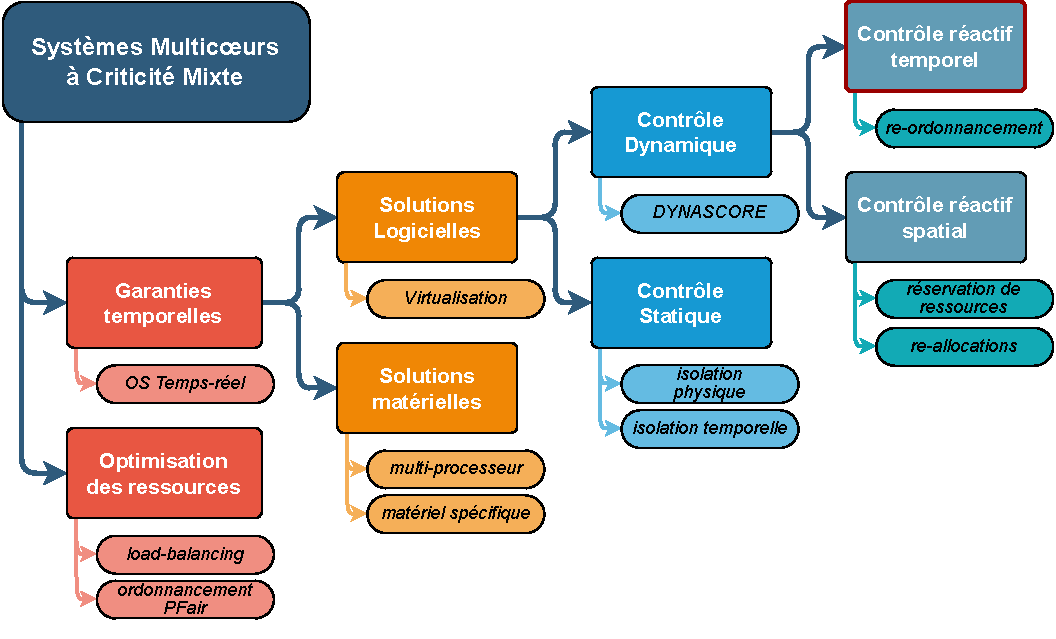
\includegraphics[width=\linewidth]{schemas/StateOfTheArt_plan}
    	\captionsetup{justification=centering}
    	\caption{Vue d'ensemble des solutions pour systèmes à criticité mixte sur calculateur multicœur}
    	\label{fig:stateoftheartsituation}
    \end{figure}

    \subsection{Solutions Matérielles et Logicielles}
    
    \subsubsection{Solutions Matérielles}
    Parmi les axes existants pour maîtriser l'exécution de systèmes à criticité mixte, le premier choix repose dans la mise en place de mécanisme d'inhibition du problème initial. Il s'agit de gérer le problème à la source en prévenant purement et simplement toute possibilité d'interférence logicielle. Il s'agit probablement encore aujourd'hui de l'option la plus répandue dans l'industrie pour sa simplicité. Cela est dû à la simplicité du résultat obtenu notamment quand il s'agit de certifier le logiciel. En étant capable de prouver que 2 logiciels de niveau de criticité différents n'entreront jamais en concurrence pour l'utilisation du matériel, les critères de sûreté de fonctionnement pour la certification sont directement atteints.
    
    Il est possible de garantir l'absence totale d'interférences soit de façon logicielle par des mécanismes de contrôle de l'exécution, soit de façon matérielle, par construction. Ainsi, le choix fondamental de l'architecture matérielle peut directement répondre au problème. De fait si l'on est en capacité d'exécuter directement le logiciel sur un support qui, par construction, ne présente aucun risque d'interférences lié au partage de ressources, alors le problème est directement évité. C'est ce que tentent de proposer des travaux comme \cite{schoeberl_towards_2011}. L'autre possibilité repose tout simplement sur ce qui est réalisé aujourd'hui dans l'automobile par exemple, en répartissant le logiciel dans plusieurs processeurs, en utilisant donc des méthodes de communication et synchronisation inter-processeur dans une architecture distribuée.
    
    C'est aussi l'approche abordée avec les calculateurs scratchpad que nous avons présenté précédemment (c.f. \hyperref[Intro:multicoeurs]{chapitre d'Introduction}), basé sur une mémoire dédiée à chaque cœur et des séparations fortes pour prévenir toute contention. L'inconvénient fondamental de ces solutions réside dans leur immuabilité. Les perspectives d'évolution sont restreintes par le matériel, à moins d'être complètement remplacé. Par ailleurs, la conception et mise sur le marché de ce type de matériel spécialisé dépend du bon vouloir des fondeurs et pose en conséquence aussi des problèmes de coûts. Il existe par ailleurs des solutions matérielles plus fines comme avec l'ajout de modules hardware dédiés qui sont directement connectés au processeur pour accomplir des tâches spécifiques \cite{solet_hw-based_2018}. 
    
    Une analyse très complète du sous-domaine des solutions matérielles peut être consultée dans la thèse de A. Blin~\cite{blin_vers_2017}.
    
    
    \subsubsection{Solutions Logicielles}
    Inversement, il est possible de réponse aux problèmes d'interférences par des solutions logicielles. C'est dans ce cadre-ci qu'une très grande part des recherches sont effectuées. De fait un grand nombre de paramètres logiciels permettent d'influer sur les performances d'exécution de tâches concourantes. On pourra citer notamment les stratégies pour~: 
    \begin{itemize}
    	\item	l'ordonnancement des tâches,
    	\item	l'allocation des tâches sur les cœurs,
    	\item 	l'accès aux ressources partagées (caches, mémoire, bus d'accès...).
    \end{itemize}

	Tous ces éléments ayant des interactions fortes entre eux, les solutions logicielles proposent à la fois une très grande variété de choix et de possibilités d'aborder la question, mais cela pose par la même la question de la complexité de réalisation qui dépendra du niveau de focalisation sur un point précis ou à l'inverse de la manipulation de tous les aspects du système. Les solutions les plus globales se retrouvant notamment dans les solutions de virtualisation \cite{augier_real-time_2006} et plus généralement des systèmes d'exploitation dédiés temps-réel (RTOS -- Real-Time OS) comme PikeOS~\cite{kaiser_evolution_2007} ou encore OSEK/VDX~\cite{bechennec_trampoline_2006} qui est un standard ayant donné lieu à plusieurs implémentations. Ces deux exemples ont donné lieu respectivement à la norme ARINC 653 dans l'avionique, et AUTOSAR Classic dans l'automobile. Le cadre offert par ces propositions ne répond a priori pas directement aux problématiques émergentes d'interférences entre les logiciels. En revanche ils proposent tous les outils d'implémentation nécessaires. Ce sont donc des technologies probablement nécessaires, mais pas suffisantes, à l'implémentation et certification de systèmes temps-réels à criticité mixte qui requièrent la mise en place de mécanismes plus spécifiques. On pourra mentionner le cas de PikeOS qui a proposé récemment la mise en place d'une structure de la plateforme opérationnelle avec allocation de ressources temporelles (plages de temps fixes) et spatiale (plages d'utilisation de chaque ressource partagée) pour l'exécution des tâches critiques et non critiques de façon à prévenir toute exécution simultanée qui pourrait engendrer des interférences entre ces deux catégories de logiciels~\cite{sysgo_ag_arinc_2019}. Cela a permis en 2013 la certification au plus haut niveau pour le ferroviaire (SIL4 de la norme EN50128)  du framework temps-réel ainsi développé pour un processeur dual-cœur. Un autre exemple de solution industrielle temps-réel qui propose du partitionnement spatial et temporel est proposé par Krono-Safe, il s'agit d'Asterios~\cite{krono-asterios-2017}. 
		
	C'est dans ce cadre que bon nombre d'études analytiques du problème sont développées. En effet, un des ressorts principaux de la maîtrise de l'exécution du logiciel réside dans le maintien d'un mode de fonctionnement nominal associé à des estimations de pire temps d'exécution (\textit{WCET -- Worst Case Execution Time}). Il s'agit des fondamentaux d'analyse des systèmes à criticité mixte, tel que présenté par \cite{vestal_preemptive_2007}. Chaque niveau de criticité pouvant être associé avec différents degrés d'exigence sur l'estimation des WCET. Sachant que plus une estimation de WCET est précise et exhaustive dans ce qu'elle prend en compte, plus ce sera complexe et coûteux à réaliser. De fait, l'estimation précise et sûre du WCET d'une tâche s'exécutant sur un processeur multicœur reste aujourd'hui un problème ouvert, encore abordé dans le cadre d'outils d'estimation analytique comme \cite{kastner_timeweaver_2019}. De ces estimations peuvent découler diverses stratégies de contrôle de l'exécution du logiciel.
	
	\subsection{Contrôle Statique et Dynamique}
	Il est possible d'établir une dichotomie parmi les mécanismes de gestion des tâches dans les systèmes à criticité mixte entre les solutions \textit{statiques} d'une part et les solutions de contrôle \textit{dynamique} d'autre part. 
	
	\subsubsection{Contrôle statique}
	Dans le cas d'utilisation de solutions statiques, les décisions d'exécution des tâches sont prévues en amont, lors de la phase de développement, pour obtenir un modèle totalement prédictif et stable d'exécution. Ils se basent donc sur la combinaison des spécifications fonctionnelles et sur des estimations de temps d'exécution moyen et pire temps pour prédéterminer un ordonnancement et une allocation statique des ressources. Cela permet d'éviter par construction l'exécution concourante de logiciels qui pourraient partager des ressources
	
	Il s'agit de ce qui est le plus communément employé, avec des surestimations nécessaire des créneaux réservés à chaque tâche de façon à garantir en toute condition le respect des exigences temporelles en évitant toute exécution parallèle indésirable. Dans l'industrie les frameworks employés se basent sur ce type de méthodes. Il y a notamment Classic AUTOSAR \cite{autosar_timing_2016} dans l'automobile peut utiliser un ordonnancement fixe, ou encore dans l'avionique avec le standard ARINC 653 \cite{prisaznuk_arinc_2008}. Toujours dans l'automobile, le réseau de communication standardisé Flexray~\cite{makowitz_flexray-communication_2006} utilise aussi une méthode d'allocation statique de créneaux de communication pour obtenir des garanties fortes sur la latence d'émission/réception des messages. En contrepartie de la forte maîtrise de l'exécution du logiciel, ces méthodes ont l'inconvénient de sur-allouer les ressources nécessaires au fonctionnement du système, et donc d'aller à l'encontre de l'objectif de maximisation d'utilisation de ces dernières.
	
	En plus des stratégies d'ordonnancement statiques qui présentent une forme d'isolation temporelle entre les tâches, il est possible de proposer de l'isolation spatiale, par le partitionnement des ressources mémoire notamment. On peut citer par exemple le travail de \cite{mancuso_real-time_2013} qui propose une méthode de profilage hors-ligne des tâches pour déterminer les pages mémoires les plus utilisées. Cela permet de contrôler la position de ces données dans les caches partagés pour limiter les interférences associées. D'autres travaux se sont intéressés plus spécifiquement à la question de l'allocation des tâches en complément d'une isolation spatiale et temporelle pour optimiser la taille des fenêtres temporelles réservées pour chaque tâche \cite{tamas-selicean_task_2011}. Enfin, certains travaux ont combiné l'utilisation de méthodes d'ordonnancement statique des tâches par exclusion d'exécution simultanée des tâches de différents niveaux de criticité avec des techniques d'isolation matérielle suivant des méthodes analytiques d'identification des interférences pour proposer une approche générale qui a pu être mise en application sur un cas avionique réel. Cette approche hybride mi-statique mi-adaptative semble présenter des résultats encourageants \cite{giannopoulou_scheduling_2013}.
	
	L'association de partitionnement temporel et spatial des tâches avec des méthodes comme celles susmentionnées permet d'obtenir les exigences nécessaires pour la sûreté des systèmes embarqués tels que décrit dans les divers standards associés. Ils permettent en revanche peu d'évolutions sans avoir à refaire tout le travail d'intégration depuis le départ. 
	
	De fait, il a été admis qu'il semble difficile, sinon impossible, de trouver une méthode qui capture les problèmes de contention dans leur ensemble dans un système multicœur avec cache partagé~\cite{suhendra_exploring_2008}. Cela mène les solutions suscitées à devoir surestimer les réservations de ressources nécessaires à l'obtention des garanties temps-réel. Ce constat nous conforte dans l'idée qu'à défaut de pouvoir contrôler et empêcher tout risque de contention dans ce type d'architecture, il est préférable d'en surveiller et contrôler les conséquences pour prévenir toute conséquence catastrophique.
	
	Il est à noter que cela ne disqualifie pas pour autant ces méthodes, qui apportent des propriétés solides. Une solution globale consistera sans aucun doute en un juste milieu entre l'usage de mécanismes statiques d'allocation et d'isolation statique des logiciels avec des mécanismes réactifs d'adaptation pour permettre malgré tout une meilleure utilisation des ressources de calcul.
	
    
	\subsubsection{Contrôle Dynamique}
    
     Survient alors la possibilité d'employer des mécanismes de monitoring pendant l'exécution de façon à pouvoir réagir à des évolutions du système qui mènent à des défaillances temporelles tel qu'un dépassement d'échéance. L'intérêt de ce type de mécanisme est de privilégier l'adaptation aux conditions de fonctionnement. Cela peut permettre une meilleure robustesse à des légères variations dans les conditions d'usage. Ces aléas de fonctionnement peuvent être de nombreuses origines, à la fois externes avec des conditions de fonctionnement qui n'ont pas été prévues (interférences électro-magnétiques, comportement utilisateur inattendu...) ou bien internes (conjonction de plusieurs évènements logiciels simultanés qui donnent un comportement imprévu). Les mécanismes réactifs sont en revanche plus complexes à concevoir pour continuer à offrir les garanties désirées et apportent forcément leur lot d'incertitudes. 
     
     \begin{figure}[ht]
     	\centering
     	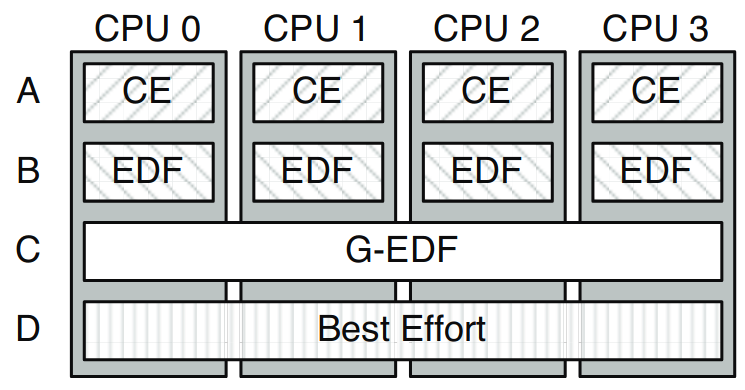
\includegraphics[width=0.7\linewidth]{schemas/MC2_scheduling_model}
     	\captionsetup{justification=centering} \caption{Allocation de conteneurs avec leurs politiques d'ordonnancement pour chaque niveau de criticité avec MC\up{2} sur un quadricœur~\cite{herman_rtos_2012}}
     	\label{fig:mc2schedulingmodel}
     \end{figure}
 
     Une des premières approches pour l'implémentation de systèmes à criticité mixte est le framework MC\up{2} \cite{anderson_multicore_2009} dont une implémentation est proposée par \cite{herman_rtos_2012}. Ce dernier propose un cadre d'implémentation pour un système à 5 niveaux de criticité\footnote{les niveaux de criticité 3 et 4 décrits ont été regroupés dans le schéma de Herman \& al.} qui disposent chacun d'un conteneur dédié ainsi que d'une politique d'ordonnancement associée tel qu'illustré dans la ~\autoref{fig:mc2schedulingmodel}. Le concept sous-jacent est de prioriser les niveaux de criticité par étage. Ainsi, la partition de plus haut niveau de criticité est exécutée en priorité, avec un ordonnancement statique selon une table préétablie (\textit{cyclic executive}). Quand aucune tâche de ce niveau de criticité n'est en attente d'exécution, les tâches du second niveau de criticité peuvent s'exécuter selon un ordonnancement pEDF (\textit{partitionned Earliest Deadline First}), c'est-à-dire priorité à l'échéance la plus proche, partitionné selon chaque cœur. De la même façon, les troisième et quatrième niveaux s'exécutent si aucune tâche des niveaux de criticité supérieurs ne sont en attente, cette fois-ci selon une politique g-EDF (\textit{global-EDF}). Et uniquement si tous ces niveaux de criticité se sont exécutés sans dépassement, alors le dernier niveau de criticité peut s'exécuter en \textit{best-effort}. 

     
     D'autres travaux ont pu montrer que du contrôle dynamique par construction de modèles prédictifs d'exécution présente aussi une bonne piste d'optimisation de l'exécution des applications sur multicœur en limitant les interférences. Des travaux comme ceux de \cite{kim_application_2019} ont pu étudier la question par l'utilisation d'un modèle par apprentissage automatique. 
     C'est par conséquent vers ce type de solutions réactives avec un contrôle dynamique de l'exécution de tâches que nous allons nous positionner. 

	\section{Mécanismes de contrôle réactif}
    Les mécanismes de contrôle réactif peuvent se focaliser sur différentes parties du système pour limiter les risques de fautes logicielles provoquées par l'exécution de logiciels concurrents. D'ailleurs rien n'empêcherait d'employer des mécanismes qui agiraient sur plusieurs composants à la fois. Les principaux éléments sur lesquels les mécanismes de contrôle agissent sont : 
     \begin{itemize}
     	\item	directement sur l'ordonnancement des tâches, par mise en pause ou changement de priorités des tâches durant le fonctionnement. Il s'agit alors d'un contrôle dynamique \textit{temporel} (c.-à-d. le \textit{moment} où s'exécutent les tâches est ajusté par rapport au fonctionnement nominal).
     	\item	sur l'utilisation du support d'exécution soit par limitation d'accès (budget d'utilisation), soit par priorisation de l'utilisation, soit par réservation d'espace dédié à certaines tâches pour les espaces mémoires notamment. Il s'agit alors d'un contrôle dynamique spatial (c.-à-d. la capacité d'accès au support d'exécution, et donc aux ressources partagées, est ajusté par rapport au fonctionnement nominal).
     \end{itemize}
 
 	\subsection{Contrôle réactif spatial}
 	Le contrôle réactif spatial repose sur la gestion des ressources partagées de façon à isoler les tâches de différents niveaux de criticité sur l'utilisation de ces dernières. Il peut s'agir d'allocation d'espace mémoire avec réservation de cache par exemple \cite{suhendra_exploring_2008}. D'autres travaux se focalisent plutôt sur les politiques d'accès aux ressources via les bus d'accès.
 	
 	En ce sens, des travaux comme ceux de \cite{blin_maximizing_2016} proposent un mécanisme de monitoring qui a été calibré hors-ligne, en amont, de façon à identifier une surcharge du système. Le cas échéant, un contrôle spatial est effectué  pour rendre l'utilisation du bus d'accès mémoire exclusif au cœur exécutant les tâches critiques pour garantir le respect des échéances sur ces dernières. La solution ici proposée est intéressante dans son approche, mais de par ses hypothèses implique une mise en pause de cœurs entiers du processeur, qui auront été alloués aux tâches non critiques. De même, \cite{yun_memory_2012} propose une régulation de la bande passante au niveau système pour chaque cœur.
 	
 	Il existe par ailleurs des mécanismes réactifs qui vont modifier l'allocation dynamique des tâches sur les cœurs pour équilibrer la charge. C'est le cas du modèle proposé dans \cite{xu_semi-partitioned_2019} qui suppose un changement de mode d'une partie des cœurs, permettant la migration de tâches non critique vers les cœurs qui sont toujours en fonctionnement nominal.
    
    \subsection{Contrôle réactif temporel}
    Nombreux sont les travaux qui réalisent du contrôle dynamique temporel, axé sur une adaptation de l'ordonnancement des tâches. Les ordonnancements dynamiques tels que les dérivés d'EDF~\cite{lelli_efficient_2011}, \cite{behera_schedulability_2012}, \cite{rodriguez_multicriteria_2013} permettent l'optimisation des ressources de calcul. La question demeure sur l'usage de stratégies d'ordonnancement globaux (l'exécution des tâches et leur allocation aux cœurs disponibles se fait à l'exécution) ou bien partitionnés (chaque cœur dispose de son propre ordonnanceur, les tâches sont allouées à chaque cœur à la conception). Ces deux grandes méthodes d'ordonnancement sont représentées dans la ~\autoref{fig:SchedulingModels}. Il existe par ailleurs des stratégies d'ordonnancement intermédiaires dites semi-partitionnées où certaines tâches sont partitionnées tandis que d'autres peuvent migrer librement entre les cœurs. Des comparaisons ont pu être étudiées entre ces types d'ordonnancement, par exemple par \cite{li_analysis_2014}. 
    %, mais n'offrent a priori pas de garanties strictes sur les contraintes temps réel.
    \begin{figure}[h!]
    	\centering
    	\begin{subfigure}{.45\textwidth} \centering
    		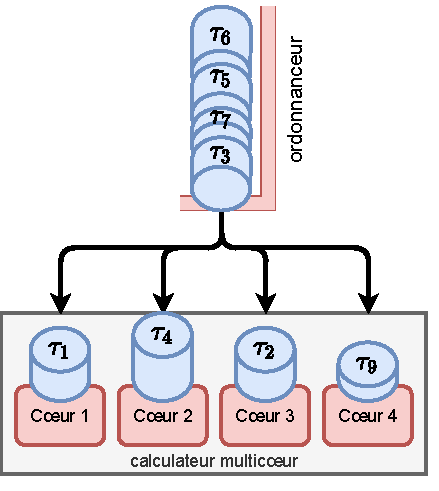
\includegraphics[width=\linewidth]{Ordonnancement_Global}
    		\caption{Modèle d'ordonnancement global}
    		\label{fig:globalScheduling}
    	\end{subfigure}
    	\begin{subfigure}{.45\textwidth} \centering
    		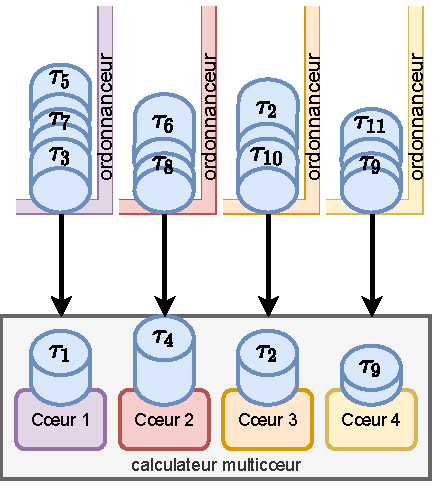
\includegraphics[width=\linewidth]{Ordonnancement_Partitionned}
    		\caption{Modèle d'ordonnancement partitionné}
    		\label{fig:partitionnedScheduling}
    	\end{subfigure}
    	\caption{Modèles d'ordonnancement}
    	\label{fig:SchedulingModels}
    \end{figure}
        
    Aussi, il est possible de disposer d'un ordonnancement des tâches différent pour plusieurs modes de fonctionnement du système. Ce dernier change donc de mode selon les besoins ou les risques. Un modèle spécifique de système à criticité mixte ainsi proposé est le modèle à \textit{criticité duale}. En d'autres termes, les tâches sont catégorisées selon deux niveaux de criticité différents. Selon les cas, on peut parler de criticité haute et basse, de tâches strictes et souples ou encore simplement de tâches critiques et non critiques. Les solutions concernées dans ces situations reposent alors sur un passage d'un mode de fonctionnement faiblement critique vers un mode de fonctionnement hautement critique où seul l'exécution des tâches de criticité haute est garantie. C'est le cas par exemple de la proposition d'amélioration de MC\up{2} avec un changement de mode dans \cite{chisholm_supporting_2017}. Dans une vision axée sur la sûreté de fonctionnement des systèmes, on peut considérer que le mode de fonctionnement faiblement critique est le comportement nominal attendu. À l'inverse, les modes plus critiques sont des modes dégradés progressifs dans lesquels certaines tâches peuvent avoir un fonctionnement non garanti, voire abandonné. Ces modes de fonctionnement ne doivent en conséquence pas constituer la règle, mais l'exception, envisagée pour les exigences de sûreté de fonctionnement. Les travaux de Trapp et al. ont eu l'occasion de s'intéresser à la pertinence d'utiliser de tels mécanismes de changement de modes \cite{trapp_runtime_2007}. Il s'agit d'un élément relativement important à mentionner dans le cadre d'une proposition de mécanisme qui apporte une garantie stricte dans des situations pire cas, en complément d'une infrastructure logicielle qui propose un cadre d'exécution de logiciel à criticité mixte avec une bonne exploitation des ressources.
    
    \begin{figure}[ht!]
    	\centering
    	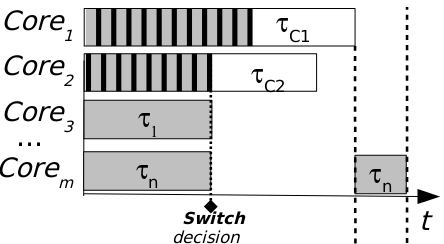
\includegraphics[width=0.7\linewidth]{schemas/DYNASCORE_tasks_sched_example}
    	\caption{Principe de contrôle d'exécution non optimisé dans \cite{kritikakou_multiplexing_2016}}
    	\label{fig:dynascoretasksschedexample}
    \end{figure}
    Dans ce sens, \cite{kritikakou_distributed_2014}, \cite{kritikakou_dynascore_2017} propose un mécanisme réactif qui se base sur deux niveaux de criticité avec le diagnostic de risque d'interférences des tâches à faible niveau de criticité sur les tâches critiques du fait du matériel partagé. La proposition consiste à surveiller l'exécution des tâches critiques de façon à identifier le moment où les interférences ne peuvent plus être tolérées, au risque de déclencher des dépassements d'échéances critiques. À cet instant-là, les tâches non-critiques sont stoppées pour prévenir le risque. La méthode de contrôle consiste à mesurer à des points de fonctionnement prédéfinis l'état d'avancement de l'exécution des tâches critiques, et de le comparer à des estimations de pire temps d'exécution restant à ce point de fonctionnement. Par calcul d'une condition de sûreté, le mécanisme de contrôle identifie le risque  pour passer en mode dégradé. Tel qu'illustré en ~\autoref{fig:dynascoretasksschedexample}, les tâches critiques $\tau_{C1}$, $\tau_{C2}$ sont exécutées sur les cœurs 1 et 2 tandis que les tâches non critiques $\tau_{1}$ [...] $\tau_{n}$ sont exécutées sur les autres cœurs. La vérification à intervalles réguliers permet d'identifier le point de décision au-delà duquel les tâches non critiques sont arrêtées temporairement pour garantir la terminaison des tâches critiques avant leur date butoir.
    

    
    Ces résultats ont été une grande source d'inspiration pour la suite de ces travaux dans le concept de surveillance de l'exécution des tâches critiques pour ne provoquer une transition dans un mode dégradé qu'en cas de dernier recours. Cela offre l'avantage d'être accessible quels que soient les autres mécanismes et méthodes employées par le système pour l'exécution des tâches, tout en offrant des garanties claires pour certaines d'entre elles. En revanche, on pourrait reprocher le fait que cette méthode requiert l'instrumentation des tâches au niveau de leur code source, ce qui n'est pas possible dans le cadre d'emploi de logiciels en boite noire.

   \section{Positionnement des travaux}
   
   Dans la vaste étendue des études sur les systèmes à criticité mixte et de sûreté de fonctionnement, nous avons proposé une classification macroscopique. Bien entendu, cette dichotomie itérative est arbitraire et certains types de mécanismes n'y sont par conséquent pas positionnables. Par exemple, il est possible de trouver des mécanismes matériels dynamiques qui se basent sur une reconfiguration matérielle en cas de faute temporelle, tel que dans \cite{lin_scheduling_2015} avec la prise en compte d'un calculateur primaire et secondaire pour le changement de mode. Ou encore le projet DREAMS~\cite{fohler_evaluation_2018} qui propose notamment une gestion dynamique des ressources en cas de surcharge du processeur. Ceci étant dit, la classification que nous proposons, agrégée dans la ~\autoref{fig:stateoftheartsituation} permet d'avoir une approche du domaine du plus global au plus spécifique par segmentation des propositions académiques en dichotomies successives. Il nous est ainsi possible de positionner notre axe d'approche dans cet ensemble et d'identifier les choix techniques et méthodologiques associés à chaque embranchement de cette vue d'ensemble.
   
   En effet, au regard des éléments précédemment mentionnés, il nous semble intéressant de trouver une solution logicielle qui soit \textit{flexible} et \textit{combinable} facilement avec d'autres techniques existantes, qui abordent potentiellement le problème sur un autre de ses paramètres. Plus spécifiquement, il devrait être possible de proposer des méthodes d'ordonnancement et d'allocation des tâches qui permet une bonne utilisation des ressources matérielles, tout en y adjoignant notre proposition qui offre des \textit{garanties sur les échéances temporelles}. 
   Ajoutez à cela la complexité d'identification et neutralisation des interférences matérielles, cela impose un \textit{mécanisme logiciel réactif} d'anticipation et mitigation des fautes qui influe sur l'exécution des tâches non critiques. 
   Aussi, il devient souhaitable de permettre un retour en fonctionnement nominal, dans les conditions où les risques de défaillances ont été écartés. 
   \\
   \smallbreak
   Par ailleurs, nous nous positionnons dans un contexte industriel où les évolutions logicielles sont constantes, avec des contraintes de coûts et de temps de développement non négligeables. Ce contexte implique aussi l'usage de logiciels en boite noire, où il n'est pas possible d'accéder et modifier le code source de façon systématique. Cela demande donc des solutions qui demandent un surcoût de développement limité en cas d'évolution (typiquement associé à le re-estimation analytique précise de pires temps d'exécution par exemple) et employable sans modification de code source.
   
   Avec la considération de tous ces éléments, notre objectif est~:
   \begin{itemize}
   	\item 	d'éviter les défaillantes temporelles par dépassement d'échéances critiques d'une part, 
   	\item   de permettre une bonne utilisation des ressources matérielles d'autre part.
   \end{itemize} 
	Ce qui peut se formaliser de la manière suivante~: 
	\begin{mdframed}[outerlinewidth=1.5pt,
	innerlinewidth=1.5pt,
	middlelinewidth=2pt,
	middlelinecolor=white,
	bottomline=false,topline=false,rightline=false]
	Comment prendre en compte les problèmes d’\textbf{interférences} sur calculateur multicœurs  pour garantir le \textbf{respect d’échéances} temporelles tout en \textbf{optimisant l’utilisation des ressources} de calcul ?
\end{mdframed}
	
	Pour répondre à cela, nous proposons un mécanisme de surveillance et de contrôle de l'exécution des tâches critiques, de façon à intervenir sur l'exécution des tâches non critiques uniquement en cas de nécessité. L'intention étant de prévenir de façon préventive et circonstancielle les interférences inter-tâches pour offrir des garanties temporelles aux tâches critiques. L'approche se voudra non intrusive sur le logiciel embarqué en abordant les tâches critiques d'un point de vue fonctionnel avec un mécanisme de contrôle bas niveau pour la surveillance et le contrôle de l'exécution.  

\ifdefined\included
\else
\bibliographystyle{StyleThese}
\bibliography{these}
\end{document}
\fi
